\section{Tutorial: Cow Tracker}
Nachdem im letzten Kapitel die Services von \gls{aws} Mobile Hub erläutert wurden, geht es jetzt darum, diese Services zu nutzen und eine kleine Android App zu entwickeln. Folgende Anforderungen gilt es mit der App umzusetzen:
\begin{itemize}
	\item Login via E-Mail/Passwort und Facebook
	\item Anzeige der Kühe eines Nutzers auf einer Karte
	\item Anzeige der aktuellen Position des Nutzers auf der Karte
	\item Zu jeder Kuh soll die Entfernung vom Nutzer angezeigt werden	 
\end{itemize}
Die Entwicklung der Android App erlaubt erste Erfahrungen mit \gls{aws} Mobile Hub zu sammeln, im folgenden werden die einzelnen Schritte beschrieben. 

\subsection{Erstellung eines Android Projekts mit Android Studio}
Der Quellcode für die Android App kann von GitHub "https://github.com/MichZipp/Playground-AWSMobileHub" heruntergeladen werden. In diesem Artikel werden lediglich die Konfigurationsschritte für das Backend erläutert. Nun öffnet man das heruntergeladene Android Projekt in Android Studio. Als nächstes konfigurieren wir unser Backend. 

\subsection{Erstellung eines \gls{aws} Mobile Hub Projekts}\label{erstellungmbprojekt}
Um ein neues Projekt anzulegen, logen wir uns bei der "\gls{aws} Console" ein und wählen den Service "Mobile Hub" aus. Dann kann dem Wizard gefolgt werden, bei dem wir den Projektnamen und die Projektplattform, in unserem Fall Android, auswählen. Standardmäßig ist Amazon Pipeline zur Analyse der Nutzerdaten aktiviert und unser Dashboard sollte wie auf Abbildung \ref{fig:mobilehubbackendoverview} aussehen. Als nächstes können wir Cloud Services hinzufügen, die wir zur Erfüllung unserer Anforderung benötigen. Jedes mal wenn wir im Dashboard neue Cloud Services hinzufügen oder Einstellung verändern, müssen wir "Intergrate" klicken, um eine neue Konfigurationsdatei zu erhalten. Diese Konfigurationsdatei fügen wir bei unserem Android Projekt unter "res/raw" ein. Wenn wir in unserer Android App auf die Cloud Services zugreifen, holt sich die \gls{sdk} automatisch die nötigen Information über den Service aus dieser Konfigurationsdatei.

\begin{figure}[h!]
	\centering
	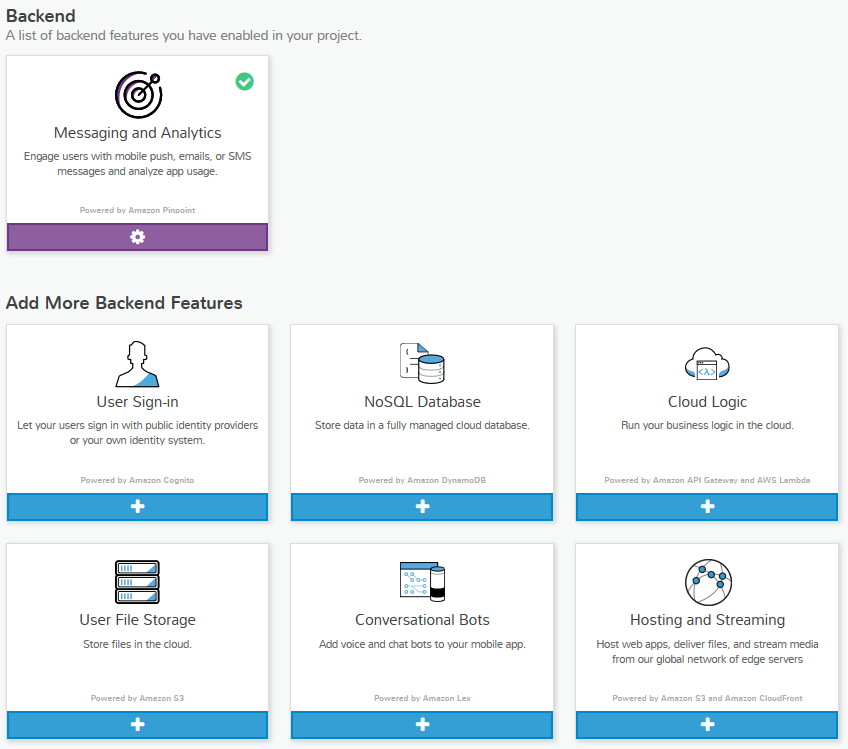
\includegraphics[width=1\linewidth]{Pictures/MobileHubBackendOverview}
	\caption[Dashboard von \gls{aws} Mobile Hub]{Dashboard von \gls{aws} Mobile Hub}
	\label{fig:mobilehubbackendoverview}
\end{figure}

\subsubsection{Login}
Ein Nutzer soll sich entweder mit E-Mail und Passwort oder Facebook authentifizieren können. 

\begin{itemize}
	\item E-Mail und Passwort:
	Dazu klicken wir in unserem Dashboard auf "User Sign-in" und wählen "E-Mail und Passwort" aus. Wir setzen das Häkchen zur Erzeugung eines neuen Benutzerverzeichnisses und legen anschließend fest, welche Anforderungen ein Passwort haben soll. Es kann festgelegt werden, wie viele und welche Zeichen das Passwort beinhalten muss. Um den Vorgang abzuschließen, klicken wir einfach "Create user pool".
	\item Facebook:
	Um Facebook als Authentifizierungsmethode zu verwenden, müssen wir zuerst uns bei der "Facebook Developer Console" anmelden und ein neues Projekt erstellen. Nach der Erzeugung des Projekts, finden wir unter "Einstellungen - Allgemeines" eine App-ID, welche wir kopieren. Nun gehen wir zurück zum \gls{aws} Mobile Hub Dashboard, klicken auf "User Sign-in" und wählen Facebook aus. Anschließend werden wir aufgefordert, die kopierte App-ID einzugeben. Ist dies erledigt, klicken wir auf "Enable Facebook Login".
\end{itemize}

Als nächstes wollen wir uns den Login in unserer Android Projekt anschauen, dazu öffnen wir die Klasse "AuthenticatorActivity" und betrachten die Methode "showSignIn()". Wir können sehen, dass sich mit nur wenigen Zeilen Code ein Login Fenster erstellen lässt, dass mit unserem Backend kommuniziert.

\subsubsection{NoSQL Datenbank}
Nun wollen wir eine Datenbank hinzufügen, in der die GPS-Daten der Kühe eines Nutzers gespeichert sind. Dazu klicken wir im Dashboard auf "NoSQL Database" und erstellen eine neue Datenbank mit dem Namen "Locations". Die Struktur der Datenbank wollen wir selbst festlegen und wählen deshalb "Costum Schema" aus. Anschließend legen wir die Datenbank Struktur wie in Abbildung \ref{fig:nosqldatabasesetup} fest und klicken anschließend "Create Table", um die Datenbank zu erstellen. Über "Download Models" kann eine Java Klasse heruntergeladen werden, die wir in unser Android Projekt einbinden. Somit können abgefragte Datensätze zu einem Java Objekt geparsed werden und wir können einfach Attribute abfragen, setzen oder ändern.

\begin{figure}[h!]
	\centering
	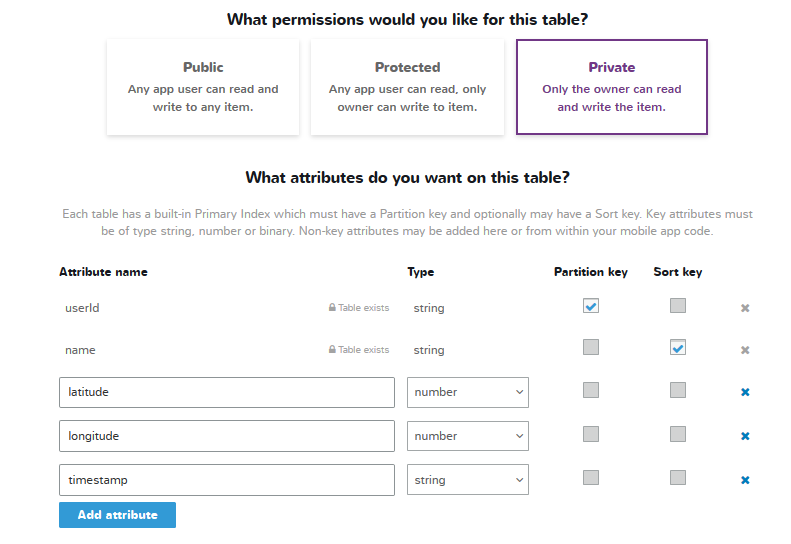
\includegraphics[width=1\linewidth]{Pictures/NoSQLDatabaseSetup}
	\caption[Datenbank Konfiguration]{Datenbank Konfiguration}
	\label{fig:nosqldatabasesetup}
\end{figure}

Schauen wir uns noch den Zugriff auf die Datenbank in der Android App an, dazu öffnen wir die Klasse "DBHandler". Durch die Methode "createLocation()" kann eine neue Position einer Kuh in der Datenbank abgespeichert werden. Mit der Methode "queryLocations()" können die Positionen aller Kühe des aktuellen Nutzers abgefragt werden. Damit wir nicht manuell neue Datensätze in die Datenbank eingeben müssen, gibt es die Methode "generateTestLocations()", die fünf Test Datensätze in die Datenbank einfügt. In der "MapsActivity" der Android App wird der "DBHandler" genutzt, um die Position der Kühe abzufragen. Diese Positionen werden dann auf einer Google Map mit einem Marker markiert. Zusätzlich wird noch via GPS der Standort des Nutzer ermittelt und ebenso mit einem Marker auf der Karte angezeigt. 

\subsubsection{Cloud Logik}
Wenn wir unsere Android App starten, haben wir bereits ein Login Fenster bei dem wir uns anmelden können und nach dem Login wird uns unsere Position und die unserer Kühe angezeigt. Nun wäre es für uns noch wichtig zu wissen, wie weit eine Kuh von uns entfernt ist. Wir gehen jetzt davon aus, dass die Berechnung der Entfernung sehr viel Ressourcen in Anspruch nimmt und wollen deshalb die Berechnung in der Cloud durchführen. Dazu klicken wir im Dashboard auf "Cloud Logic" und anschließend auf "Create a new \gls{api}". Wir füllen das Formular wie in Abbildung \ref{fig:cloudlogicsetup} aus und erstellen die \gls{api} mit "Create \gls{api}".

\begin{figure}[h!]
	\centering
	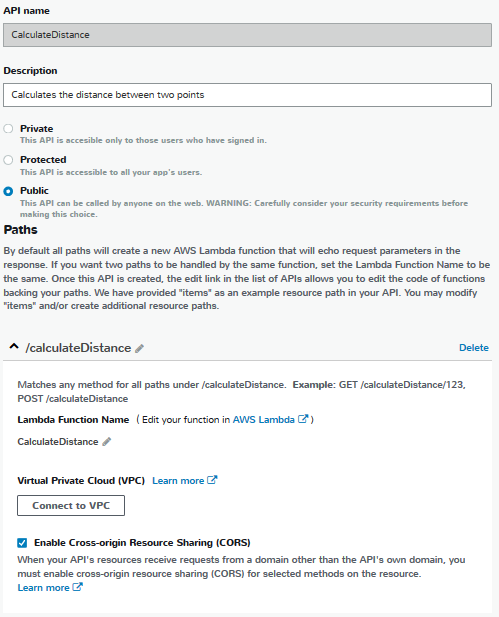
\includegraphics[width=1\linewidth]{Pictures/CloudLogicSetup}
	\caption[Cloud Logik Konfiguration]{Cloud Logik Konfiguration}
	\label{fig:cloudlogicsetup}
\end{figure}

Es wurde automatisch eine Lambda Funktion generiert, um diesen Vorgang prüfen, wählen wir den Service "Lambda Function" in unserer \gls{aws} Console aus. Wenn alles funktioniert hat, sollten wir eine Lambda Funktion mit dem Namen "CalculateDistance" sehen. Nun können wir unseren Quellcode für die Berechnung der Entfernung hinzufügen. Standardmäßig kann im Browser mit JavaScript entwickelt werden, wir bevorzugen aber Java und nutzen dafür die \gls{ide} Elipse mit dem \gls{aws} Plugin, um den Code später in die Cloud hochladen zu können. Als erstes nutzen wir das \gls{aws} Plugin um eine neues Java Lambda Projekt zu erstellen, anschließend fügen wir den Quellcode aus dem Ordner "CowTrackerLambda" unseres heruntergeladenen Git Repository ein. Nun müssen wir den Quellcode nur noch hochladen, dazu machen wir ein Rechtsklick auf das Projekt und klicken auf "Amazon Web Services - Upload function to lambda...". Es öffnet sich ein Wizard, bei dem wir die Lambda Funktion auswählen müssen, dementsprechend wählen wir "CalculateDistance" aus und klicken auf "Upload". Und schon haben wir Cloud Logik zu unserer Android App hinzugefügt. Die Cloud Logik wird in der Klasse "DistanceCalculator" der Android App über ein HTTP Anfrage abgerufen. 

\subsection{Ergebnis}
Nun haben wir alle nötigen Schritte beendet, um unsere Anforderung umzusetzen. Starten wir die App, können wir uns einloggen und die App zeigt eine Karte mit unserer Position und der Position der Kühe. Klicken wir auf einen Marker, so zeigt es uns den Kuhnamen und unsere aktuelle Entfernung zu dieser Kuh an. Abbildung \ref{fig:cowtracker} zeigt zwei Screenshots, wie das Login-Fenster und die Kartenansicht aussieht. 
\begin{figure}[!ht]
	\centering
	\begin{subfigure}{0.49\linewidth}
		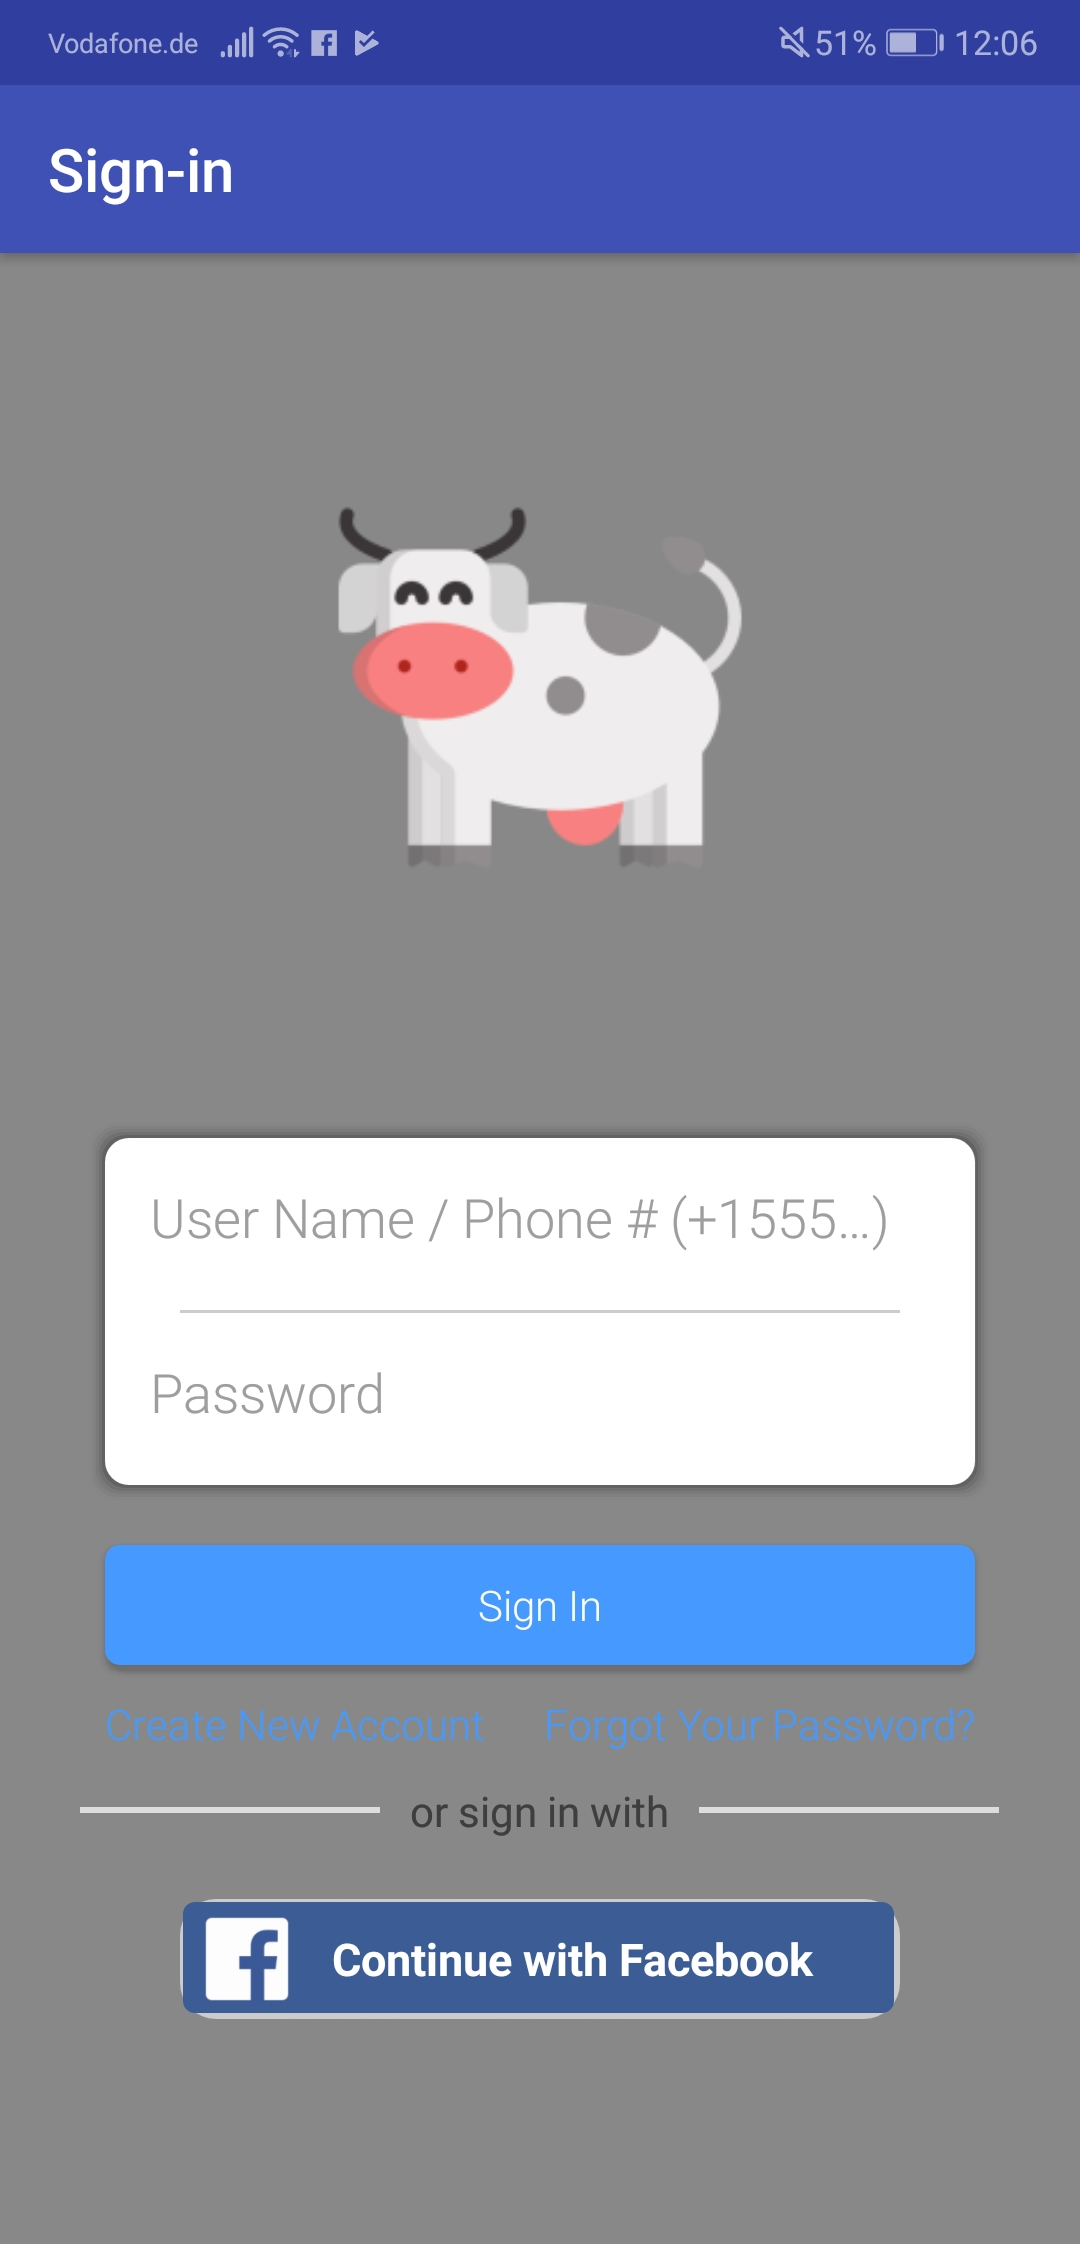
\includegraphics[width=1\linewidth]{Pictures/Screenshot_Login.jpg}
		\caption{ }
		\label{subfig:cowtracker_login}
	\end{subfigure}
	\begin{subfigure}{0.49\linewidth}
		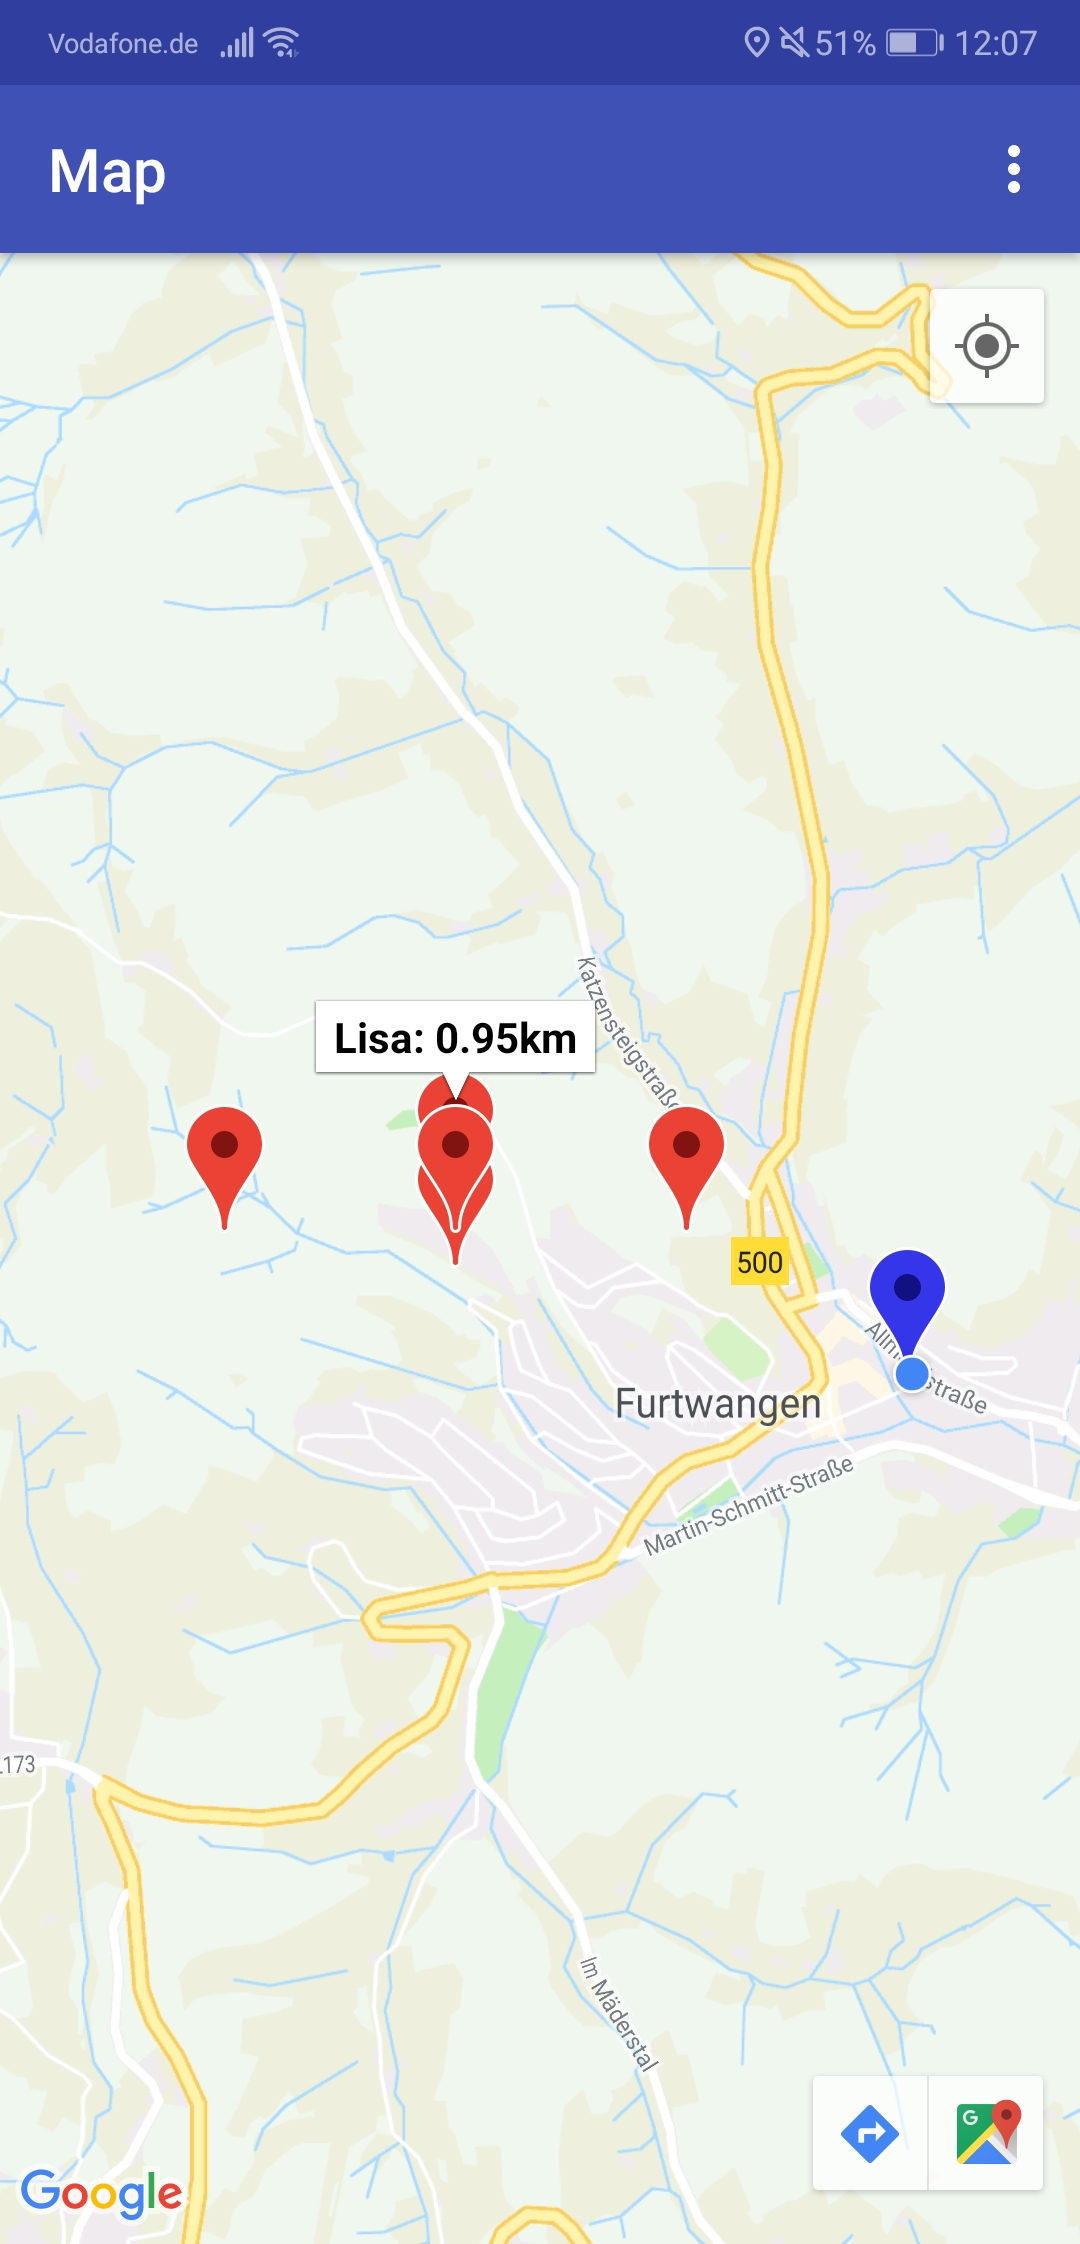
\includegraphics[width=1\linewidth]{Pictures/Screenshot_Map.jpg}
		\caption{ }
		\label{subfig:cowtracker_map}
	\end{subfigure}	
	\caption{Screenshots der Cow Tracker Android App}
	\label{fig:cowtracker}
\end{figure}

Als nächsten wollen wir noch einen kleinen Einblick in die Nutzungsstatistik werfen. Dazu wählen wir in der \gls{aws} Console den Service Pinpoint und anschließend unser Projekt aus. Nun werden uns jede Menge Statistiken zu unserer Android App angezeigt. Abbildung \ref{fig:pinpointanalystics} zeigt uns einen kleinen Ausschnitt davon. Es wird uns beispielsweise angezeigt, wie viel Nutzer die App starten oder sich pro Tag einloggen.

\begin{figure}[h!]
	\centering
	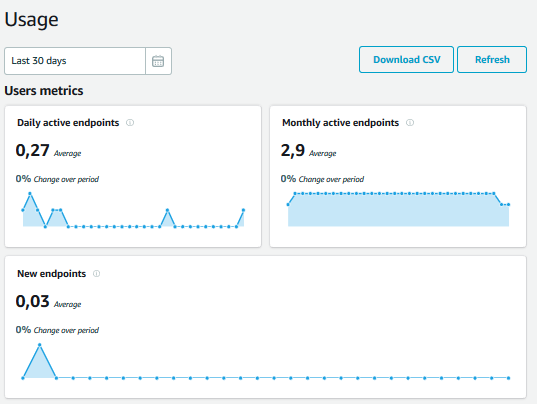
\includegraphics[width=1\linewidth]{Pictures/PinpointAnalystics}
	\caption[Pinpoint Nutzungsanalyse]{Pinpoint Nutzungsanalyse}
	\label{fig:pinpointanalystics}
\end{figure}
